\chapter{COMMUNICATION \& AUTHENTICATION}\label{cha:auth} \index{authentication}
Because just about all devices that are connected to a network are one way or another connected to the Internet you can bet that they find themselves in an untenanted or malicious environment. Everything connected to the Internet is very likely to be hacked. Thus, authentication is needed for remote sensing devices to communicate. \cite[]{auth:M2Mcom}\\
In this chapter will show ways of authentication (two factor, M2M and biometric) that is in the area of this thesis. The biometric part is in the area because it has good ways of measure strength in a biometric trait (especially fingerprint) that will be used when comparing strength of my tests of characteristic noise in the mobile device.

\section{Two factor authentication}\label{sec:2fauth} \index{two factor authentication}
There are more ways to authenticate a user than password, however it is the most common. There are three different types of authentication; 
\begin{itemize}
	\item Something the authenticator \textit{have} like a key, card, passport and so on
	\item Something the authenticator \textit{knows} for example password
	\item Something the authenticator \textit{are}, known as biometrics such as fingerprint or iris pattern
\end{itemize}
\cite[p.~31]{rosssec} \\
Authentication in two factor means a combination of two of the three types of authentication above. An example can be use of a credit card (you have) in combination with a PIN-code (you know) to collect the money from an ATM. Something the authenticator have and knows is the most common combination. The third one, cost is the biggest reason form that biometrics isn't that common yet.
\cite[p.~47]{rosssec}

\section{Challenge-Response authentication}\label{sec:challResp} \index{challenge-response}
The challenge-response protocol is build upon the idea that the user to a system first must complete a challenge decided by the system in order to access the system. An example is modern car keys when trying to start the engine, the engine controller give the key an challenge consisting of a random $n$-bit number. The key encrypt the challenge and response. \\
The problem challenge-response protocols facing is often to achieve good randomness, thus is the challenge not random enough there is a risk for malicious user to calculate the $n$-bit number. \\
There are other applications than looks, like the HTTP Digest Authentication. It uses the authentication process  which a web server challenges a client or a proxy with the common secret of a password. The server sends nonce to the client or proxy, whom hash the nonce with the password and the requested URI. This authentication mechanism is not vulnerable to password snooping and is used in cases like; client-server-authentication in SIP or the protocol for Voice-Over-IP telephony. This protocol however is vulnerable to man-in-the-middle. \\
\\
Ross states however that a much more visible use of challenge response is in \textit{two-factor authentication} (~\sectionref{sec:2fauth}). An example of use is if you have and bank card reader when accessing your bank on the Internet. When you want to log in there are an random challenge of $n$ numbers. You put these numbers together with a PIN into your bank card reader. The reader encrypts these numbers (pin + $n$ numbers) using a secret key shard with the sever of the bank. The fist $n$ numbers of the encryption is displayed on the card reader and you enter this in the login screen as a password. 
\begin{figure}[H]
	\centering
    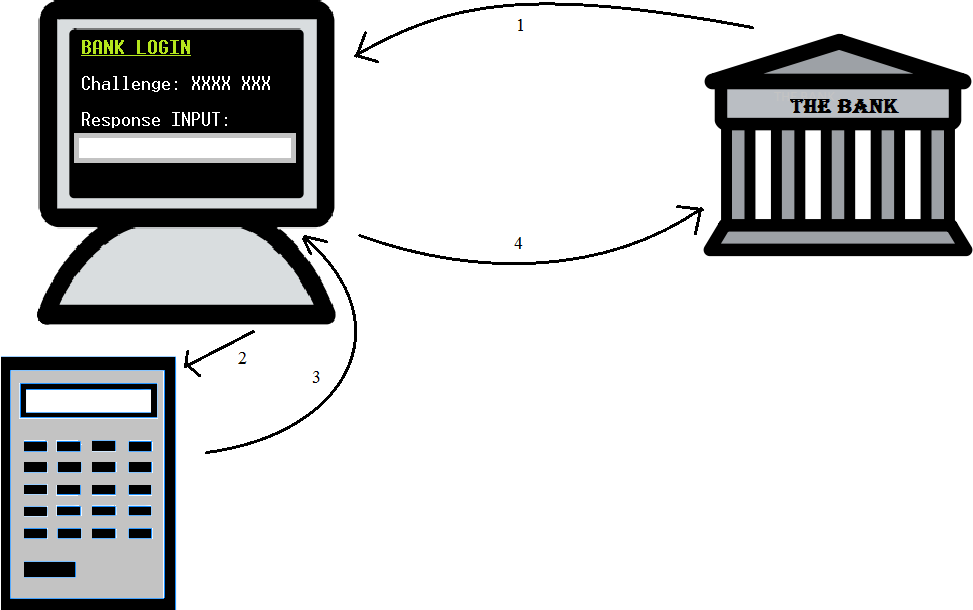
\includegraphics[scale=0.3]{img/challenge-response-bank}
    \caption{Challenge-response authentication with bank card reader}
  \label{fig:challengeResponse}
\end{figure}
Describing of~\figureref{fig:challengeResponse}:
\begin{enumerate}
	\item Bank sending Challenge XXXX XXX to the requesting address.
	\item User enter PIN and XXX XXX in the bank card reader.
	\item The reader encrypts the PIN and number with a secret key shared with the bank. The first numbers of the encryption is displayed o the reader. ($YYYY YYY = {XXXX XXX, PIN}_k$) 
	\item The user enter the encrypted numbers YYYY YYY on the log in screen and sends it as a password to the bank.
\end{enumerate}
~\cite[ch.3]{rosssec}

\section{M2M\index{M2M} (Machine-to-machine)}\label{sec:m2mauth}
Information that is exchanged via a communication network between machines has to establish conditions for doing so, that is where M2M is used. M2M is often a short synonym for M2M communication, meaning the communication conditions between devices. M2M communication is only the communication made between machines without any human behind it. A mobile device interacting with a call center application is not M2M, cause there is a human behind the mobile device calling. The reason for that using mobile devices in this thesis is that they have many hardware parts that can be used for no human communication with other devices (see chapter ~\ref{cha:character}). These hardware parts can be found in other simpler devices such as accelerometer sensor probe that also can be applied on the result.
\\
Often is M2M involving similar devices  in the same M2M area network, interacting with an application. This makes it possible for devices to access public networks as well, via a gateway or router. An example is the heating system in smart homes. 
Devices are not a new thing, but when we have a growing world of IoT devices with very specific characteristics is growing. Thus makes the area of M2M more important to make these devises talk without a human behind. This affecting the requirements on the application and networks dealing with the devices. Characteristics of this devices is listed blow;
\begin{itemize}
	\item[] \textbf{Multitude}, they say that connected devise not directly interacting with humans, the big part of IoT is soon to be significant more than the ones which interact directly with humans. This will put more pressure on application and networks dealing with all devices.
	\item[] \textbf{Variety} of connected devices with requirements like data exchange rate, form factor, computing, or communication capabilities. M2M applications have to be built, in order to define and develop common enabling capabilities.
	\item[] \textbf{Invisibility} meaning that the device has virtually zero human control. The more invisibly the less likely for error caused by humans. 
	\item[] \textbf{Criticality} devices that can harm humans like voltage. Therefor reliability is an important factor. 
	\item[] \textbf{Intrusiveness} many of the increasing connected devices raise the privacy question like refrigerators, stoves, doors, etc.
\end{itemize}
All this devices with no human control is like told above very different, but many of them is similar in some ways, such that the functionality is limited, low-powered, embedded and have long life cycles. The fact that they often are embedded makes it hard to separate between M2M communication and machine-to-human or human-to-human communication.
\cite[p.~2-4]{m2mComm}

\subsection{Difference between M2M and IoT}
Internet-of-Things, meaning to making everything connected to everything in the Internet. IoT is now in its starting pits and ready to start the race. Machine-to-machine communication is a part of that, but it also covers other areas and IoT some that M2M doesn't. The common denominator is according to Polsonetti \textit{remote device access}, where the embedded hardware modules in a machine that communicate wireless or not is M2M applications. Remote device access for IoT has a much more wider perspective that not only including same device communication but also passive and other low-power sensors that not can be motivated as a M2M hardware module.
\cite[]{cpM2MIoT}\\
In this thesis is M2M a subset of IoT, since it always one mobile device that wants to authenticate then it can communicate with other deceives.

\subsection{M2M authentication}
There are no standardized way of authenticate in M2M, but effort is done in the area. An example is \cite[]{auth:M2M} where he based authentication on a machines fingerprint. But this fingerprint isn't of the same character as the one this thesis is focusing on. In his article the fingerprint consist of hardware message of computers, such serial number of CPU, MAC address of network card, Machine ID etc. These things have through the years been proven to bee pretty easy to spoof. There are hundreds of guides of how to do that in many platforms like mobile devices (iPhone \cite[]{spoofMaciPhone} and Android \cite[]{spoofMacAndriod}) that is the thesis area. \\
Like \cite[]{auth:M2Mcom} that states in their article that ``\dots traditional methods such as “what you know and who you are” may not be applied''. But the aim in section~\ref{sec:aim} is to do precisely that and with the advantage that using ``regular'' authentication that is more  tried and tested. Thus the next section will be about biometric systems and how they authentication which is used for who you are.


\section{The biometric process}\label{sec:biometric}
\begin{center}\textit{``A biometric system measures one or more behavioral characteristics...information of an individual to determine or verify his identity.''} \cite[p.~3]{introbio}\end{center}

\subsection{Recognition}
As said before is biometric something you \textit{are} and the person who wants to be recognized to the system. Buy, showing his or her biometric identifier (fingerprint, iris, DNA, etc.) to the biometric system, thus seen as a \textit{user} of the system. The strength in biometrics is also the fact that it knows if a user is known to the system even if the user denies it. \cite[ch.~1]{introbio}

\subsection{Biometric systems}
There are some blocks for building a biometric systems, which can measure characteristics of a user. In biometric these characteristics is called \textit{traits, indicators, identifiers, or modalities}, but for for the aim of this thesis will it still be called characteristics. For designing, implementation and evaluation when building a biometric system there are some steps that has to be done;\\
\\
The first step is to collect biometric data and store it in a database with the users identity. The recognition is then done by again collect biometric data from the user and compared to the database. This is the so called \textit{enrollment and recognition phase}. The raw biometric data is often destroyed after enrollment and the recognition is all about pattern matching. This matching is done in four steps;
\begin{enumerate}
	\item \textit{Sensor -} to collect the raw biometric samples, that can be a image, amplitude signal, online signature, odor or chemical-based.
	\item \textit{Feature extractor -} first has to make the raw biometric samples comparable, mostly done in three pre-process operations; 
	\begin{itemize}
    	\item Quality assessment, is the sample good enough?
		\item Segmentation, remove background noise from sample
		\item Enhancement, by using an algorithm to improve the sample 
    \end{itemize}
	\item \textit{Database -} that has the data from the enrollment phase together with some identity data (like name orID). This database should having a access control mechanism for security reasons.
	\item \textit{Matcher -} where the sample from the enrollment is compared with the sample in recognition, to see if it's a match or not. This is done by having a match score to decide how close the enrolled and recognition sample is. The score is counted in different way depending on the characteristics that is used in the system. 
\end{enumerate}
\cite[ch.~1]{introbio}

\subsection{Biometric authentication}
Biometrics authentication, is sometimes also called verification that answers the question ``Are you the one you say you are?''. There is also biometric identification that answers ``Are you someone known to the system?'' but that is not what this thesis aim to answer. The practical difference between authentication and identification is that the user has to give the system some kind of information (username, passport, email etc.) on who they claim to be. But in identification the user just give the sample to the system, which then looks if the user is known to the system or not. The identification look-up takes longer time since you look for all samples in the database and compare them, in authentication you only look for the claimed identity. \cite[ch.~1]{introbio}

\subsection{Measurements}
Biometric measurements is a bit more tricky than in a password-based system where the answer just is `match' or `no match'. The accuracy of the biometric system must be consider when you choose characteristics. This is measured by two rates \index{FRR} (False Reject Rate) that is the probability that two samples from the same user is not a match and \index{FAR} (False Accept Rate) is the probability that two samples from different users is a match. A match is decided authentic between two samples from the same user is high enough and as a \textit{impostor} is there is similarity between two samples from different users.  \\
There are a threshold $\eta$ that is used to decide the FRR and FAR. The proportion of authentic scores ($\omega_{1})$) that are less than $\eta$ is defined as FRR and the impostor score ($\omega_{0})$) that are greater than or equal to $\eta$ is FAR. Which can be described mathematical as; 
$$ FAR(\eta) = p(s\geq \eta | \omega_{0}) = \int_{\eta}^{\infty} p(s | \omega_{0}) ds, $$
$$ FRR(\eta) = p(s\geq \eta | \omega_{1}) = \int_{-\infty}^{\eta} p(s | \omega_{1}) ds, $$
where $p(s\geq \eta | \omega_{x})$ us the probability density function of the authentic respective impostor score. 
\cite[p.~18]{introbio}

\subsection{Design a biometric system}
When designing a biometric system it is done in a five activity cycle. Depending on the outcome of one activity, the next step could be forward or redoing earlier activity. The design cycle is represented as a flow-chart below (from page 27 in \cite[]{introbio}), followed by a description of the five activities. \\
\\
\textbf{Understand nature of application -} is about deciding functionality type and classified based on how well the system fits this six different behaviors; cooperative, overt, habituated users, attended, untenanted operation, controlled operation and open system. The first is if the user will be \textit{cooperative} or not, like if the user wants to access something it is likely to cooperate. \textit{Overt} is if the user knows that it is object for biometric recognition. If the user interacts with the system a lot it is likely that the user will be \textit{habituated}. The enrollment and recognition operations can either be \textit{attended} by a human or not. The environment of the operations may have to be \textit{controlled} in terms of temperature, pressure, etc. in order to work. Last there are also the question if the system will be closed or \textit{open}, such if the database of biometric data will be shared between applications or be in one closed application.) \\
\\
\textbf{Choose biometric characteristics -}\label{auth:bio:character} is also classified, based on seven different factors. The thing with biometrics is that it will never be completely solid, thus all the factors can't be perfect. Counted to this is that the factors will have different value for different systems.
\begin{enumerate}
	\item \textit{Universality,} the fail-to-enrollment (FTE) rate should be low.
	\item If the \textit{uniqueness} of the characteristics is high will the rate of FAR be low. 
	\item The characteristic should be high in terms of \textit{permanence} and not be changing significantly over time.
	\item \textit{Measurability} from the user perspective in terms of collecting characteristics, should convenient.
	\item The time of the authentication is measured in \textit{performance}.
	\item User should have a high \textit{acceptability} in present their characteristics to the system.
	\item \textit{Circumvention}, in terms of how easy it is to malicious fake the characteristics.
\end{enumerate} 

\textbf{Collect biometric data -} is apart from the collecting also includes factors of time, cost and size of the equipment.\\
\\
\textbf{Choose features and matching algorithm -} is a critical step since this is the heart of the system and has to bee done with a great deal of knowledge if the selected characteristics and the data extracted from it. \\
\\
\textbf{Evaluate the biometric system -} by asking different questions. There are no framework for doing this and it has to account different perspective as require experts of different field such psychology, business, computer science and statistics. There exists no framework for these types of evaluation but \cite[]{introbio} propose doing it in three evaluation-stages technology, scenario and operational.

\begin{figure}[!ht]
	\begin{tikzpicture}[node distance=1.6cm]
	\node (start) [justtext] {Start};
	\node (understand) [process, below of=start] {Understand nature of application};
	\draw [arrow] (start) -- (understand);
		
	\node (choose) [process, below of=understand] {Choose biometric characteristics};
	\draw [arrow] (understand) -- (choose);
		
	\node (collect) [process, below of=choose] {Collect biometric data};
	\draw [arrow] (choose) -- (collect);
	\node (coll) [right of=collect, xshift=1.3cm] {};

	\node (algorithm) [process, below of=collect] {Choose features and matching algorithm};
	\draw [arrow] (collect) -- (algorithm);
	\node (alg) [right of=algorithm, xshift=1.3cm] {};

	\node (evaluate) [process, below of=algorithm] {Evaluate the biometric system};
	\draw [arrow] (algorithm) -- (evaluate);

	\node (end) [justtext, below of=evaluate] {End};
	\draw [arrow] (evaluate) -- (end);

	\node (req) [justtext, text=blue, left of=understand, xshift=-3cm, yshift=-1cm] {Performance requirements};
	\draw (understand) -| (req);
	\draw [->,>=stealth] (req) |- (evaluate);
		
	\node (knowledge) [justtext, text=red, left of=algorithm, xshift=-1.5cm] {Prior knowledge};

	\draw [arrow, draw=red, very thick] (knowledge) |- (algorithm);

	\draw [dashed] (evaluate) -| (alg);
	\draw [darrow, dashed] (alg) -- (algorithm);
	\draw [dashed] (alg) -- (coll);
	\draw [darrow] (coll) -- (collect);
	\draw [darrow] (coll) |- (choose);
\end{tikzpicture}
	\caption{\label{fig:biodesigncycle} The design cycle of a biometric system}
\end{figure}